\documentclass[11pt]{article}
% \usepackage{nodalida2019}
\usepackage{natbib}
\usepackage{times}
\usepackage{todonotes}
\usepackage{tabularx}
\usepackage{tikz}
\usetikzlibrary{arrows,automata}

\usepackage{stmaryrd}
\usepackage{enumitem}
\usepackage{newunicodechar}
\input{PaperTools/latex/newunicodedefs}
\usepackage{hyperref}

\title{A Wide-Coverage Symbolic Natural Language Inference System}

% - Two-phase system (Dyn semantics from theorem proving)
% - Anaphora (as in Jolli paper) --- but this is the first time that this is done for FraCas.
% - Multiple readings
% - Threshold-based interpretation of (some) adjectives + Linear arithmetic proofs
% - New handling of prepositions and adverbs
% - Definites handled by adding an assumption at the top-level. (instead as inline existential) -- Enabled by dyn. semantics
% - Plurals/Quantifiers improved
% - Genders are properties of nouns
% - Handling of comparatives (with threshold BUT not those of adjectives), relying largely on the dyn. semantic system

\newlist{lingex}{enumerate}{3}
\setlist[lingex,1]{parsep=0pt,itemsep=1pt,label=(\arabic*),resume=lingexcount}
\newcommand\onelingex[1]{\begin{lingex}\item #1 \end{lingex}}


\begin{document}

\maketitle{}

\begin{abstract}
  We present a system for Natural Language Inference which uses a
  dynamic semantics converter from abstract syntax trees to Coq
  types. It combines the fine-grainedness of a dynamic semantics
  system with the powerfulness of a state-of-the-art proof assistant. We evaluate the system on all sections of the FraCaS test
  suite, excluding section 6. This is the first system that does a
  complete run on the anaphora and ellipsis sections of the FraCaS. It
  has a better overall accuracy than any previous system.
\end{abstract}
\section{Introduction}
Natural Language Inference (NLI) is the task of determining of whether
an NL hypothesis H follows from an NL premise(s) P. NLI has received a
lot of attention in the Computational Semantics literature and has
been approached using a variety of techniques, ranging from logical
approaches
\citep{bos:2008,Mineshima:2015,Abzianidze:2015,bernardy_type_2017},
all the way to the recent Deep Learning (DL) models for NLI. The
latter approaches, following a general trend in NLP, have been
dominating NLI and a number of impressive results have been
produced \citep{kim:2018,radford:2018,liu:2019}.\footnote{These are
  the three systems with the best results on SNLI in increasing
  order at the time of writing.}  State-of-the-art DL systems achieve an accuracy of around
0.9 when tested on suitable datasets. However, the datasets that are
used are assuming a definition of inference that can be thought to be
`looser' or less precise compared to the definition assumed in
platforms based in logical approaches \citep{bernardy:2019}. For example, consider the following
 example  from the SNLI dataset, predominatly used to test DL
approaches:
%
\begin{lingex}
\item % An SNLI example \\
  \label{ex:snli}
\textbf{P}  A  man selling donuts to a customer during a world
exhibition event held in the city of Angeles. \\
 \textbf{H}  A woman drinks her coffee in a small cafe.\\
\textbf{Label: Contradiction} [SNLI]
% \item % An example from FraCaS\\
% \textbf{P1} A Scandinavian won the Nobel Prize.\\
% \textbf{P2}	Every Swede is  Scandinavian.\\
% \textbf{Q}  Did a Swede win the Nobel prize? \\
% \textbf{H} A Swede won the Nobel prize.\\
% \textbf{Label: Yes} [FraCaS 173]
\end{lingex}
%
In \ref{ex:snli}, a number of non-trivial
assumptions have to be made in order to arrive at a contradiction: a) the two
situations described have to be taken to refer to the same situation
in order to judge that the latter  contradicts the former, b)
the indefinite article in the premise has to be identified with the
indefinite article in the hypothesis. (Additionally considering that a
person cannot be a man selling donuts and a woman drinking coffee at
the same time.) While this can be part of the reasoning humans
perform, it is not the only possibility. More precise, logical
reasoning is also a possibility, and will render the above label as unknown. Furthermore, reasoning can get very fine-grained 
as the Contained Deletion ellipsis example \ref{ex:acd} below shows:

\begin{lingex}
\item
    \label{ex:acd}
\textbf{P1}	Bill spoke to everyone that John did [elliptic V2].\\
\textbf{P2}	John spoke to Mary.\\
\textbf{Q} 	Did Bill speak to Mary?\\
\textbf{H} 	Bill spoke to Mary. \\ \textbf{Label:	Yes} [FraCas 173]
\end{lingex}

% \begin{lingex}
% \item % An example from FraCaS involving fine-grained reasoning\\
% \textbf{P1}	Bill spoke to everyone that John did.	\\	
% \textbf{P2}	John spoke to Mary.	\\
% % \textbf{Q} 	Did Bill speak to Mary?\\
% \textbf{H} 	Bill spoke to Mary.\\
% \textbf{Label:	UNK} [FraCaS 065] 	\end{lingex}


For this reason, and despite the dominance of DL approaches in pretty
much all NLP tasks, logical approaches continue to be
developed and evaluated on datasets like the FraCaS test suite and the
SICK dataset \cite{marelli:2014}.  \citet{bernardy:2017} define a
correspondence between abstract syntax parse trees of the FraCas
examples, parsed using the Grammatical Framework (GF,
\citet{Ranta:GF}), and modern type-theoretic semantics that are output
in the Coq proof assistant (the FraCoq system).  The accuracy is 0.85
for 5 sections of the FraCaS test suite. The \textsc{Langpro} system
presented by \citet{Abzianidze:2015} is based on a Natural Logic
tableau theorem prover. It achieves an accuracy of .82 on the SICK
dataset.

In this paper, we concentrate on this sort of fine-grained, logical
reasoning. In particular, we present a logic-based system that deals
with many linguistic phenomena \emph{at the same time}. It is the
first system covering the sections on ellipsis and anaphora in the
FraCaS test suite and has the best coverage and accuracy on the
overall test suite.
% This is listed below; we can let the reader figure it out.

In sum our contributions are as follows:
\begin{itemize}
\item A two-phase system (rather than a one-phase as described by
  \citet{bernardy_type_2017}): a) using Haskell as a converter between
  Grammatical Framework trees and Coq types, b) using various type
  combinators to reach the desired NL semantics.
\item The first run of the Anaphora and Ellipsis sections of the
  FraCaS (based on work by \citet{bernardy_jolli})
 \item  More coverage than any previous logical approach
 \item State-of-the-art results in terms of accuracy compared to all
   previous approaches, for every section of the FraCaS
  \item Handing of multiple readings
  \item  Threshold-based interpretation of (some) adjectives plus Linear arithmetic proofs
  \item New handling of prepositions and adverbs compared to the
    earlier system in \citet{bernardy_type_2017}, as well as new
    handling of definitions, enabled by the dynamic semantics system.
  \item Improvement over the previous treatment of Plurals/Quantifiers
  \item Big improvement on the comparatives section enabled by
    handling comparatives using a threshold (BUT one different to the
    one used for adjectives). Again, the dynamic semantics system is
    crucial here.
\end{itemize}

\section{Background}

\paragraph{GF}
In GF, abstract syntax is comprised of: a) a number of syntactic
categories, and b) a number of syntactic construction functions. The latter
provide the means to compose basic syntactic categories into more complex
ones.  For example, consider the constructor: $AdjCN : AP \to CN \to CN$. This  expresses
that one can append an adjectival phrase to a common noun and obtain
a new common noun. Furthermore,  GF is equipped  with a library of mappings from abstract
syntax to the concrete syntax of various natural languages.
These mappings can be inverted by GF, thus offering parsing from natural text into abstract syntax.
However, in this project we skip the
parsing phase and use the parse trees constructed by \citet{Ljunglof:2012},
thereby avoiding any syntactic ambiguity. 

\paragraph{Coq}
Coq is an interactive theorem prover (proof assistant) based on the
calculus of inductive constructions (CiC), i.e.  a lambda calculus
with dependent types.  Coq is a very powerful reasoning engine
that makes it fit for the task of NLI, when the latter is formalized
as theorem proving task. It supports
notably dependent typing and subtyping, which are instrumental in
expressing NL semantics.

\paragraph{Dynamic Monadic Semantics}
Dynamic Monadic Semantics have been proven to be an effective way of
dealing with anaphora and ellipsis. There are a number of approaches
using monads or other equivalent constructions (e.g. continuations as in the work of
\citet{de2006}) for anaphora and ellipsis
\citet{Shan:2002,unger:2011,Barker:04,de2016,charlow:2017}. In this
paper, we follow the approach described in
\citet{bernardy_jolli}. More details are given in the next
section.



\section{Overview of the system}

Our system consists of two main parts.
\begin{enumerate}[noitemsep]
\item A converter from syntax trees to types. The syntax trees follow
  the GF formalism, and the types follow the Coq formalism. The
  converter itself is a Haskell Program, which implements a dynamic
  semantics and comprises the bulk of our system.
\item A number of type-theoretical combinators, that encode semantical
  aspects which have no influence on the dynamic part. Such aspects
  include the treatment of adjectives (intersective, subsective, etc.)
  and adverbs (veridical or not).
\end{enumerate}

The architecture is represented schematically in Figure \ref{fig:overview}.
\begin{figure*}
  \centering
{
  \tiny
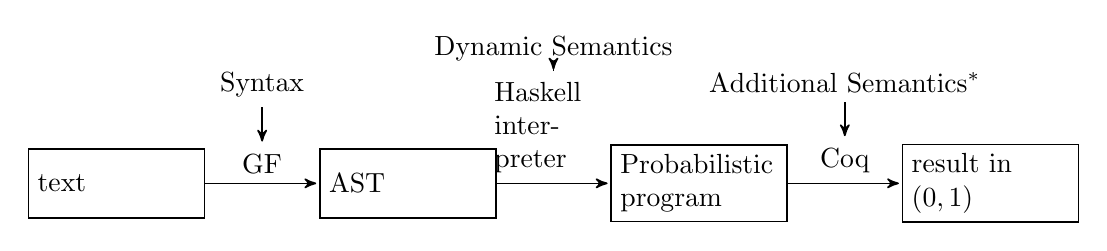
\begin{tikzpicture}[->,>=stealth',shorten >=1pt,auto,node distance=3.7cm,
                    semithick]
  \tikzstyle{every state}=[draw=black,text=black,shape=rectangle,text width=2cm]

  \node[state]         (txt)                {text};
  \node[state]         (ast) [right of=txt] {AST};
  \node[state]         (pp)  [right of=ast] {Probabilistic program};
  \node[state]         (res) [right of=pp] {result in $(0,1)$};

  \path (txt) edge              node (GF)  {GF}                  (ast)
        (ast) edge              node (Hask) [text width=1.5cm]{Haskell interpreter} (pp)
        (pp) edge               node (Coq) {Coq} (res);

  \node (Syntax) [above of=GF,node distance=1cm] {Syntax};
  \node (Sem) [above of=Hask,node distance=1cm] {Dynamic Semantics};
  \node (Hyper) [above of=Coq,node distance=1cm] {Additional Semantics$^\ast$};

  \path
  (Syntax) edge (GF)
  (Sem) edge (Hask)
  (Hyper) edge (Coq);
\end{tikzpicture}
}
\caption{Phases in our system. ($\ast$) At the level of Coq, we handle
  the details of the adverbial (veridicality properties) and
  adjectival semantics (division into subsective, extentional,
  non-committal, etc. categories.) }
  \label{fig:overview}
\end{figure*}

All the underlying systems (GF, Haskell, Coq) are based on lambda
calculi with types. We take advantage of typing, ensuring that each
translation preserve typing, locally:
\begin{enumerate}[noitemsep]
\item Every GF syntactic category $C$ is mapped to a type noted $\llbracket{}C\rrbracket{}$.
\item GF Functional types are mapped compositionally : $\llbracket{}A \to B\rrbracket{} = \llbracket{}A\rrbracket{} \to \llbracket{}B\rrbracket{}$
\item Every GF syntactic construction function ($f : X$) is mapped to a function $\llbracket{}f\rrbracket{}$ such that $\llbracket{}f\rrbracket{} : \llbracket{}X\rrbracket{}$.
\item GF function applications are mapped compositionally: $\llbracket{}t(u)\rrbracket{} = \llbracket{}t\rrbracket{} (\llbracket{}u\rrbracket{})$.
\end{enumerate}
Because all systems embed the simply-typed lambda calculus, ensuring
type-preservation locally means that types are preserved globally.
Therefore, we are certain that every GF syntax tree can be mapped to
Haskell, and eventually Coq, without error.

The dynamic semantics follows a monadic structure, as pioneered by
\citet{Shan:2002}. There are two kinds of effects carried by the
monad.  The first one comprises a series of updates and queries of
stateful elements.  There is one piece of updateable state for every
element which can be referred to by anaphoric expressions. These can
be the usual ones (like NPs), but also less usual ones (like 2-place
verbs, or a quantity --- which we illustrate below). The other kind of
effects is \emph{non-determinism}. We use non-determinism to model the
property that linguistic expressions can have several
interpretations. The monadic structure allows to locally express that
a given expression has several meanings; the monadic bind ensures that
all combinations of meanings are considered at the top-level,
combinatorially. This dynamic semantics allows us to model many
phenomena in a precise way.

\paragraph{Anaphora} Thanks to the above system, we can handle many
anaphoric cases, including E-Type and Donkey anaphora. Indeed, even
objects which have no syntactic representation can be added to the
environment. We follow here the general monadic semantics approach as outlined by
\citet{unger:2011}. However, we use a more general scope-extension
mechanism, which allows us to support examples like  the following:
\begin{lingex}
\item
    \label{ex:anaphora-scope}
\textbf{P1}	Every committee has a chairman.\\
\textbf{P2}	He is appointed its members.\\
\textbf{H} 	Every committee has a chairman appointed by members of the committee. \\ \textbf{Label:	YES} [FraCaS 122]
\end{lingex}
In the above example, the pronoun ``he'' is allowed to refer to the
object quantified over by ``every'', whose scope is extended
accordingly.

\paragraph{Ellipsis} Ellipsis is handled in essentially the same way
as anaphora. This method is made especially straightforward thanks to
using GF syntax trees, which require an explicit argument for each
predicate. Thus, ellipsis are made explicit by the parsing phase. Such
ellptic expressions are handled in the same way as anaphora.
%
For example, in \ref{ex:acd}, the argument of ``did'' is
explicitly marked as an elliptic V2, which we resolve to ``speak'' in
that context.

\paragraph{Definites} A naive way to handle definites is using an
existential type. However, if the semantics does not feature a
dynamic element, then the existential quantification is introduced
locally. This means that the quantifier can be introduced in the wrong
Context. Consider the phrase ``everyone pets the dog''. The structure
of the interpretation would be
$\forall{} x. person(x) \to \exists{}y. dog(y) \wedge pet(x,y)$.
%
Instead, our take is that definites should be treated as an anaphoric
expression with an implicit referrent. That is, if the referent is not
found in the discourse, then it will be forcibly introduced, using an
existential type, \emph{at the top-level} of the expression. To be
able to do this, we record all definites without referent, using
another portion of the environment (using a monadic effect).
For the
above example, we obtain the desired interpretation:
$\exists{}y. dog(y) \wedge (\forall{}x. person(x) \to pet(x,y))$.

\paragraph{Phrasal comparatives}
Previous attempts to tackle the section of the FraCaS test suite
devoted to comparatives showed that handling them is not easy. Our
strategy here is to leverage our dynamic semantics, revealing an
anaphoric element of comparatives. Indeed, consider the hypothesis of
(FraCaS 239): ``ITEL won more orders than APCOM lost.''  We postulate
that this sentence is equivalent to the following two separate parts:
``APCOM lost zero or more orders. ITEL won more orders [than some
elliptic quantity].''  A quantity is introduced every time we talk
about some quantity (indexed by a CN, in this case ``orders''), and it
can be referred to by a comparative, later in the discourse. Using
this idea, we can go one level deeper in the interpretation of our
example: ``APCOM lost $\theta$ orders. $\theta$ $\ge$ 0.  ITEL won at least $\theta$+1
orders.''. We see here how the quantities are introduced. They are
added to the environment so that, they can be referred to as elliptic
quantity expressions.\footnote{The degree parameter assumption is not new in the formal semantics literature \cite{Cresswell:1976,Heim:2001,Kennedy:2007,chatzikyriakidis:2017} among many others. The specific details and computational implementation, however, are.}
%
Finally, ``more'' is systematically intepreted as ``at least
<elliptic quantity>+1''. This treatment, which we illustrated here on
an example, is systematic in our implementation.


\paragraph{Adjectives}
We interpret gradable adjectives using a pair of a
measure $m : objects \to Z$ and a threshold $\tau : Z$, where $Z$ is
treated as an abstract ordered ring by Coq. (This structure has no
dynamic aspect in our model, and thus is entirely handled within Coq.)
For subsective adjectives, $\tau$ will additionally depend on the class
of the object in question. This structure has the benefit that
opposite adjectives can be easily represented (measures are opposites
$\forall{}x. m_1 x = \lnot m_2 x$ and thresholds do not overlap $\tau_1 + \tau_2 >
0$). Formalization aside, this idea is reminiscent of degree-based
approaches to gradable adjectives of
\citet{Cresswell:1976,Kennedy:2007}.  Additionally
adjectival predicates, as present in the FraCaS suite, are interpreted as
linear inequations in $Z$. Solving systems of such inequations is
decidable.
Indeed, the tactic that Coq offers for this purpose can
solve all such problems in the FraCaS suite, automatically.


\paragraph{Adverbs}
Another point, of minor theoretical importance but major practical
one, is our handling of adverbial phrases. We interpret adverbs (and
in general all adverbial and prepositional phrases) as VP-modifiers:
$Adv = VP \to VP$, where $VP = object \to Prop$. However, applying adverbs
to verb-phrases heavily complicates the Coq proofs, because such
phrases can contain quantifiers. Therefore, we instead move the
adverbs, so that they apply to (atomic) verbs only. Proofs can then be
simplify accordingly.


\section{Results and evaluation}

We evaluated FraCoq against 8 sections of the FraCaS test suite, for a
total of 259 cases. We excluded only section 7, ``temporal reference''.
The reason for
doing so is that, in our view, it contains too many examples which
require \textit{ad-hoc} treatment, and thus makes little sense to
include without complementing it with a more thorough suite which
captures a more complete landscape of the phenomena that section 7
touches.

FraCaS classifies each problem as either entailment (YES),
entailment of the opposite (NO) or no entailment (UNK).  In this work,
we have amended the FraCaS suite to correct a few problems. First,
certain test case are not formed correctly. Those were already
identified by \citet{maccartney:2007} as such (using an ``undef''
labelling), and we removed those. Second, a few test cases occur twice
in the suite, but with two different labellings (one YES and one UNK),
with an annotation that those labellings correspond to different
readings. However, elsewhere in the suite, if a problem has several
readings but only one has entailment, it occurs only once and is
marked as YES. To make the test suite consistent, if one reading
yields entailment we have always considered it as YES. We have also
removed case 199 (which appears to be vacuous). Finally we changed the
labelling of 6 cases
%(SC: Shall we remove this to the supplementary material and just say to have a look at how we amended the suite?)
% the cases listed in Table \ref{tab:overrulings},
which appeared to have been
misclassified. We note that the majority of the mistaken
classifications occur in sections 3 and 4, which have not been
previously attempted and thus, we propose, have not been properly
scrutinized. In terms of comparison, this only has a minor effect, since our system is the first system to run sections 3 and 4. 
\begin{table}
  \centering
  \small
\begin{tabularx}{\columnwidth}{ccp{3.8cm}}
 test case & new class & comment \\ \hline
    005 & UNK & missing hypothesis: there are italian tenors \\
   056 &  Yes & Already identified as such by MacCartney \\
  069 & Unk & Mary could have used someone else's workstation \\
  119 & Unk & \textit{ibid.} \\
  181 & Yes & for the same reason as 180 \\
  226 & Yes &
\end{tabularx}
  \caption{Overruled FraCaS cases}
  \label{tab:overrulings}
\end{table}

Our system classifies a case as YES if a proof can be constructed from
the premises to the hypothesis, NO if a proof of the negated
hypothesis can be constructed and UNK otherwise. Because we work with
a non-decidable logic, one cannot \emph{in general} conclude
decisively that no proof exists. Thus, we consider here that no proof
exists if it cannot be constructed with reasonable effort. In
particular, we test at the minimum that the automatic proof search
built in Coq does not succeed before classifying a problem as UNK.\footnote{The other way this can be done is by introducing a timeout as \citet{Mineshima:2015} have done.}


%  ------ Section 1
% complete: 74/74   []
% correct: 71/74   [13,14,46]
% score: 0.9594594594594594
%  ------ Section 2
% complete: 33/33   []
% correct: 27/33   [84,91,94,95,109,111]
% score: 0.8181818181818182
%  ------ Section 3
% complete: 27/28   [137]
% correct: 24/27   [124,126,127]
% score: 0.8571428571428571
%  ------ Section 4
% complete: 47/52   [171,172,191,193,195]
% correct: 45/47   [170,188]
% score: 0.8653846153846154
%  ------ Section 5
% complete: 20/20   []
% correct: 19/20   [216]
% score: 0.95
%  ------ Section 6
% complete: 29/31   [244,245]
% correct: 27/29   [242,250]
% score: 0.8709677419354839
%  ------ Section 7
% complete: 0/67   [251,252,253,254,255,258,259,260,261,262,263,264,265,266,267,268,269,270,271,272,273,274,275,277,278,279,280,281,282,283,284,285,286,287,288,289,290,292,293,294,295,296,297,298,299,300,301,302,303,304,306,307,311,312,313,314,315,316,317,318,319,320,321,322,323,324,325]
% correct: 0/0   []
% score: 0.0
%  ------ Section 8
% complete: 8/8   []
% correct: 6/8   [326,333]
% score: 0.75
%  ------ Section 9
% complete: 13/13   []
% correct: 12/13   [346]
% score: 0.9230769230769231
%  ------ Section 0
% complete: 251/259   [137,171,172,191,193,195,244,245]
% correct: 231/251   [13,14,46,84,91,94,95,109,111,124,126,127,170,188,216,242,250,326,333,346]
% score: 0.8918918918918919

\providecommand\forcecenter{\multicolumn{1}{c}}
\providecommand\ncases[1]{{\ensuremath{^{#1}}}}
\begin{table}[hbt]
  \centering
  \small
\begin{tabularx}{\columnwidth}{Xr@{\,\,}r@{\,\,}r@{\,\,}r@{\,\,}r@{\,\,}r}
Section      & {\kern -2em} \#cases & Ours     & FC & MINE & Nut  & Langpro  \\ \hline
Quantifiers  & 75          & .96  & .96    & .77  & .53  & .93  \\
             &             & \ncases{74}     &        &      &      &     \ncases{44} \\
Plurals      & 33          & .82      & .76    & .67  & .52  & .73 \\
      &          &       &     &   &   & \ncases{24} \\
Anaphora     & 28          & .86      &   -    & -    & -    &  -       \\
Ellipsis     & 52          & .87      &   -    & -    & -    &  -       \\
Adjectives   & 22          & .95 & .95    & .68  & .32  & .73 \\
             &          &  \ncases{20} &     &   &   &  \ncases{12} \\
Comparatives {\kern -1em}& 31          & .87      & .56    & .48  & .45  &  -       \\
Temporal     & 75          &  -       &   -    &   -  &  -   &  -       \\
Verbs        & 8           & .75      &   -    & -    & -    &  -       \\
Attitudes    & 13          & .92      & .85    & .77  & .46  & .92  \\ 
    &          &       &     &   &   & \ncases {9}  \\ \hline
Total        & 337         & .89      & .83    & .69  & .50  & .85  \\
             &             & \ncases{259}    & \ncases{174}  & \ncases{174}& \ncases{174}& \ncases{89}
  \end{tabularx}
  \caption{Accuracy of our system compared to others.
    ``Ours" refers to the approach presented in this paper. When a
    system does not handle the nominal number of test cases (shown in
    the second column), the actual number of test cases attempted is
    shown below the accuracy figure, in smaller font.  ``FraCoq''
    refers to the work of \citet{bernardy_type_2017}. ``MINE" refers
    to the approach of \citet{Mineshima:2015}, ``NUT" to the CCG
    system that utilizes the first-order automated theorem prover
    \textit{nutcracker} \cite{bos:2008}, and ``Langpro"
    to the system presented by \citet{Abzianidze:2015}. A dash
    indicates that no attempt was made for the section. }
  \label{tab:results}
\end{table}

Table \ref{tab:results} shows a considerable improvement over earlier
approaches in terms of coverage, with three more sections covered over
previous approaches. We thus cover 259 out of 337 cases (77\%),
compared to at most 174 cases (52\%) in previous work. Additionally,
our system performs generally the best in terms of accuracy. In
particular, section 6 largely improves in accuracy, which we
attribute to our dynamic semantics analysis of comparatives.

\paragraph{error analysis}
Our system fails to correctly classify  28 cases out of 259.  We give
here a summary of the missing features which are responsible for the failures. The  biggest source of error is 
incomplete handling of group readings. (FraCaS
013, 014, 046, 084, 111, 124, 126, 127, 137, 171, 172, 191, 193, 195, 243, 250, 333, 346). These
are cases where  a syntactic conjunction of individuals is treated as a
semantic group, or where precise counting of the members of a group is
necessary.  Other problematic cases include definite plurals with
no  universal readings (091, 094, 095). Additionally,
neither measure phrases (242) nor attributive comparatives (244, 245)
are handled.


\section{Conclusions and Future Work}
We presented a system converting GF trees to Coq types using dynamic
semantics. The system outperforms the state of the art in logical
approaches when tested on the FraCaS  and is the only system
to date to perform a run on the FraCaS ellipsis/anaphora section. The system is precise enough to form the start of a 
precise NL reasoner for controlled domains. In the future, we plan to
extend the system to cover the remaining section of the FraCaS
(tense/aspect), and also develop a more applied version to perform
reasoning on controlled NL domains.

\bibliography{PaperTools/bibtex/jp,phorae,IWCSbib,NLI}

\bibliographystyle{acl_natbib}

\end{document}